% Auto-generated diagnostic evidence. Safe to cite only as mechanism characterization.
\subsection{Pre-campaign information-geometry diagnostics}
The feeder has 583 measurements and
491 states.  Under perfect information,
$\lambda_{\min}(G_\infty)=5.68769$ and the condition
number is 4.402e+09.  The numerical implementation
returns $u^\lambda=0$ and $u^{\mathrm{tr}}=0$ at this limit, as required
by the reduction property.  These results characterize the mechanism and do
not constitute confirmatory detection performance. Removing the most
influential telemetry channel reduces weakest-direction information by
21.6\%, while removing the top eight leaves only
4.86e-13 of the perfect-information floor. Across all static
patterns, expected availability and exposure have Spearman correlation
-0.741; this collinearity is reported because it can
make a null incremental-geometry result protocol-induced rather than
substantive.

\begin{figure}[!t]
\centering
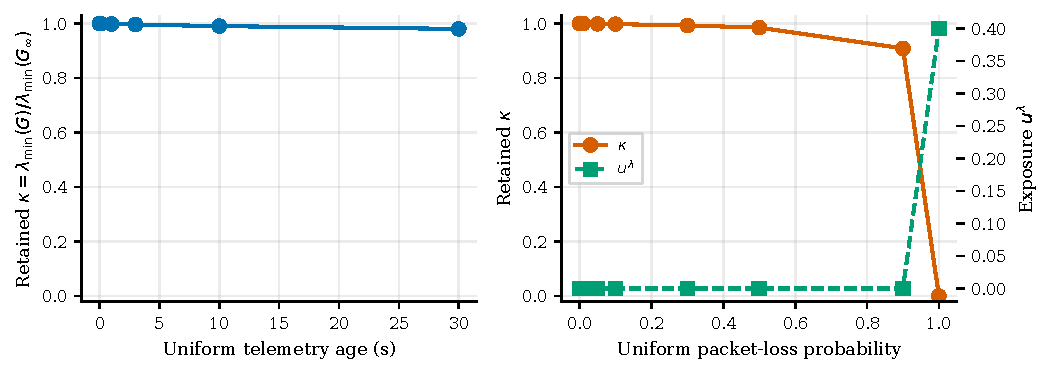
\includegraphics[width=\columnwidth]{paper1_generated/figures/fig_diagnostic_age_loss_response.pdf}
\caption{Static response to uniform age and loss. The abrupt endpoint at total loss is the observability cliff; smooth degradation away from the cliff is weak for this feeder.}
\label{fig:diagnostic-age-loss}
\end{figure}

\begin{figure}[!t]
\centering
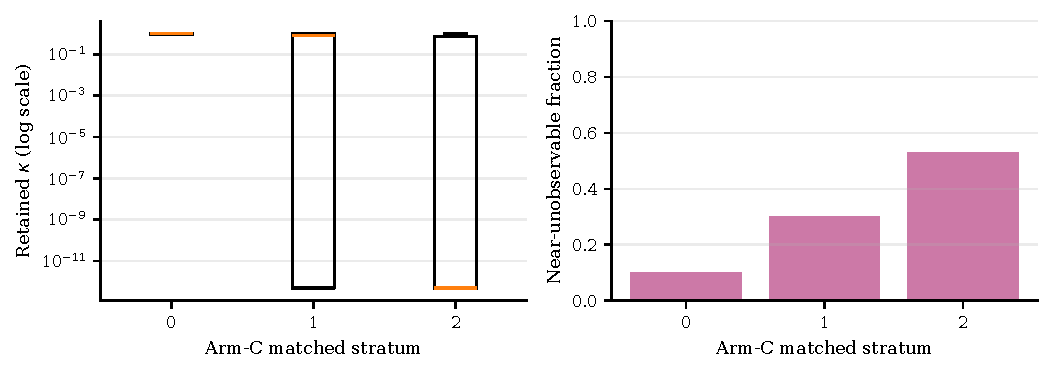
\includegraphics[width=\columnwidth]{paper1_generated/figures/fig_diagnostic_matched_identity.pdf}
\caption{Arm-C matched-count/age diagnostic. Measurement identity produces orders-of-magnitude variation in retained weak-direction information within the same trivial communication stratum.}
\label{fig:diagnostic-identity}
\end{figure}

\begin{table}[!t]
\caption{Pre-campaign Arm-C geometry diagnostic at matched received fraction and mean age. These are mechanism checks, not confirmatory detector-performance results.}
\label{tab:diagnostic-arm-c}
\centering\scriptsize
\setlength{\tabcolsep}{2.5pt}
\begin{tabular}{rrrrrr}
\toprule
Stratum & Events & $B_1$ & $B_2$ (s) & Median $\kappa$ & Near-unobs. \\
\midrule
0 & 100 & 0.822 & 0.533 & 0.993 & 10.0\% \\
1 & 100 & 0.644 & 1.067 & 0.776 & 30.0\% \\
2 & 100 & 0.467 & 1.600 & 4.9e-13 & 53.0\% \\
\bottomrule
\end{tabular}
\end{table}


\begin{figure*}[!t]
\centering
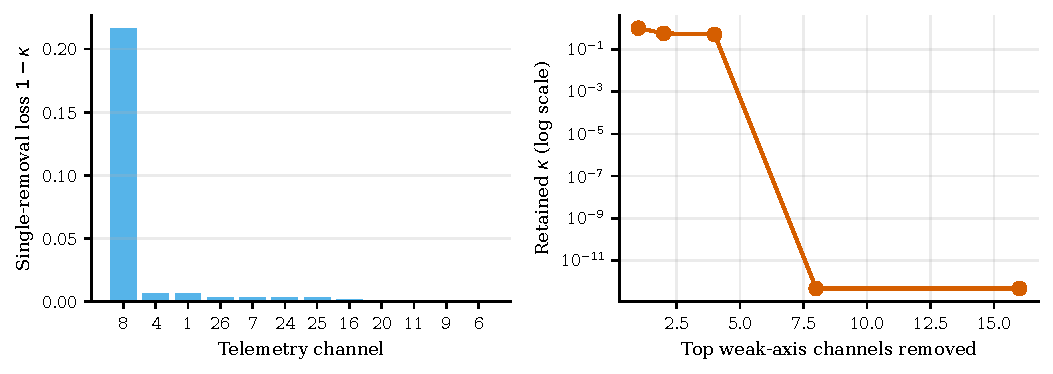
\includegraphics[width=0.88\textwidth]{paper1_generated/figures/fig_diagnostic_channel_influence.pdf}
\caption{Measurement-identity sensitivity of the weakest information direction. Left: single-channel removal loss. Right: retained information after cumulative removal of the most influential channels.}
\label{fig:diagnostic-channel-influence}
\end{figure*}

\begin{figure}[!t]
\centering
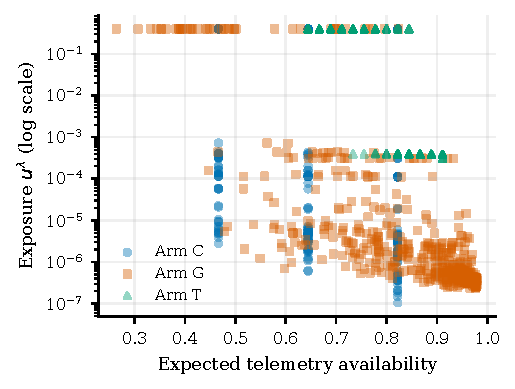
\includegraphics[width=\columnwidth]{paper1_generated/figures/fig_diagnostic_collinearity.pdf}
\caption{Static availability--exposure relationship by experimental arm. The strong but imperfect association motivates reporting collinearity and matched-pair fraction before interpreting F3.}
\label{fig:diagnostic-collinearity}
\end{figure}
